\section{Experimental Results}
\subsection{Experiment Settings}
In this section, we compare three models for PV modules in terms of accuracy and speed. These models are the Ground Truth (GT) model, the Colony-Wise (CW) model, and the N-Colony (TC) model. Without losing generality, we assume that all the cells that have the same shading level within one PV module tend to cluster together.

We use notations from Section II (Equation \ref{equ:slRepresent}) to represent the multilevel shading settings. In the experiment, we assume $SLs = \{2A, 1.75A, 1.5A, 1.25A, 1A\}$. In order to simulate multiple shading scenarios, we define a ration array that consist three configurations:
$ratios1 = \{70\%, 10\%, 5\%, 5\%, 10\%\}$,
$ratios2 = \{50\%, 10\%, 10\%, 10\%, 20\%\}$ and
$ratios3 = \{20\%, 20\%, 20\%, 20\%, 20\%\}$. The three $ratios$ cover low shading, medium shading and high shading respectively. For one PV module, we generate $100$ random shading patterns under each ratio configuration to evaluate three models.

We instantiate three different PV modules in our experiment: $60s2p$, $30s4p$ and $40s2p$. As for the bypass diode configuration, every $15$ to $20$ cells have one bypass diode according to \cite{bp1}. Therefore, $60s2p$ module has $3$ bypass diodes for each chain, and other two modules have $2$ bypass diodes for each chain. We use the same solar cell's One-Diode model parameters as in \cite{oneD1}. Diode quality factor $N_o=1.5$, diode saturation current $I_{s_o}=10^{-6}A$, serial resistance $R_{s_o}=0.0079\Omega$ and shunt resistance $R_{sh_o} = 5000\Omega$. The bypass diode has the quality factor $N_{bp_o} = 1$ and saturation current $I_{sbp_o}= 10^{-6}A$.

The circuit simulations are conducted in HSPICE \cite{hspice}. The experiment was conducted on a laptop that has an Intel $i5$ $2.4$GHz CPU, and $8$GB memory.

For the N-Colony model, $20$ shading patterns are used to curve fit the weighting factors in Equation \ref{equ:cfObj}. The curve-fitted parameters are used to validate the PV module models through the rest of shading patterns. We implement the gradient descent search to achieve the curve fitting. In order to jump out of the local optimal, several randomized initial points are used and we pick the best results. The curve-fitted parameters of the NC model are shown in Table \ref{table:ncCurveFit}. Although they are different for different PV modules, the curve fitting overhead is reasonable because in a solar farm, the types of PV modules are usually small and fixed.

Furthermore, from Table \ref{table:ncCurveFit}, $\alpha$ is always larger than $\beta$ and $\gamma$ under all conditions. This shows that $C_R$ has a larger impact on PV module modeling than $c_r$. $C_R$ is the dominant factor in a PV module��s output power. This implies that the PV module generates less power, when the shade covers more colonies while the area of the shade remains the same. Similar observations can also be found in other references \cite{villalva2009comprehensive, oneD1, oneD3}.


\subsection{Accuracy Comparisons Among the Three Models}



To evaluate accuracy of the Colony-Wise model and the N-Colony model, the average relative error of the Maximum Power Point (MPP) and the average P-V curve correlation (CORR) are compared with the Ground Truth model. The MPP represents the operation point of a PV module, and the CORR shows the similarity between the estimated P-V curve and the Ground Truth curve.

\begin{figure}[tb]
    \centering
    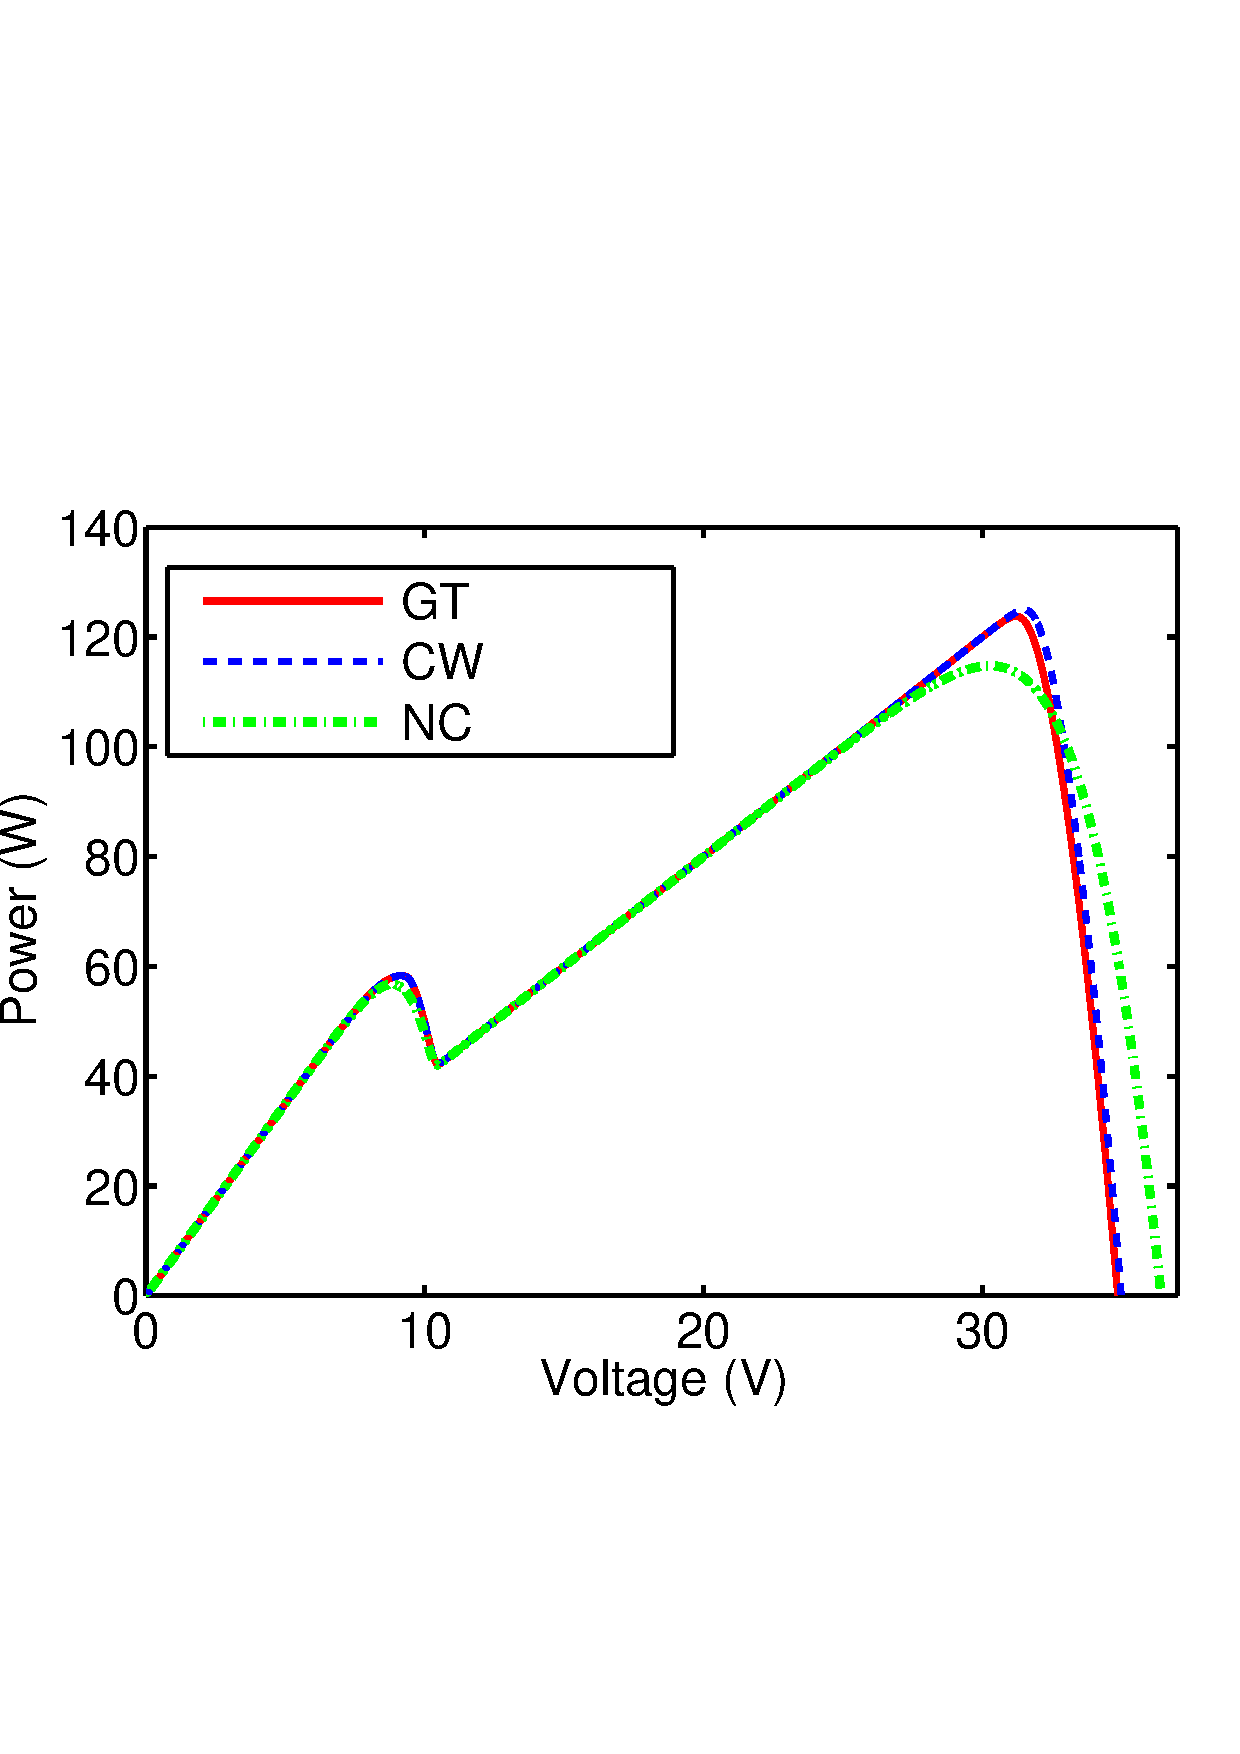
\includegraphics[width=0.8\columnwidth]{figs/pvExample.pdf}
    \caption{An example of three P-V curves generated by three models of a same PV module configuration}
    \label{fig:pvExample}
\end{figure}

\begin{figure}[tb]
    \centering
    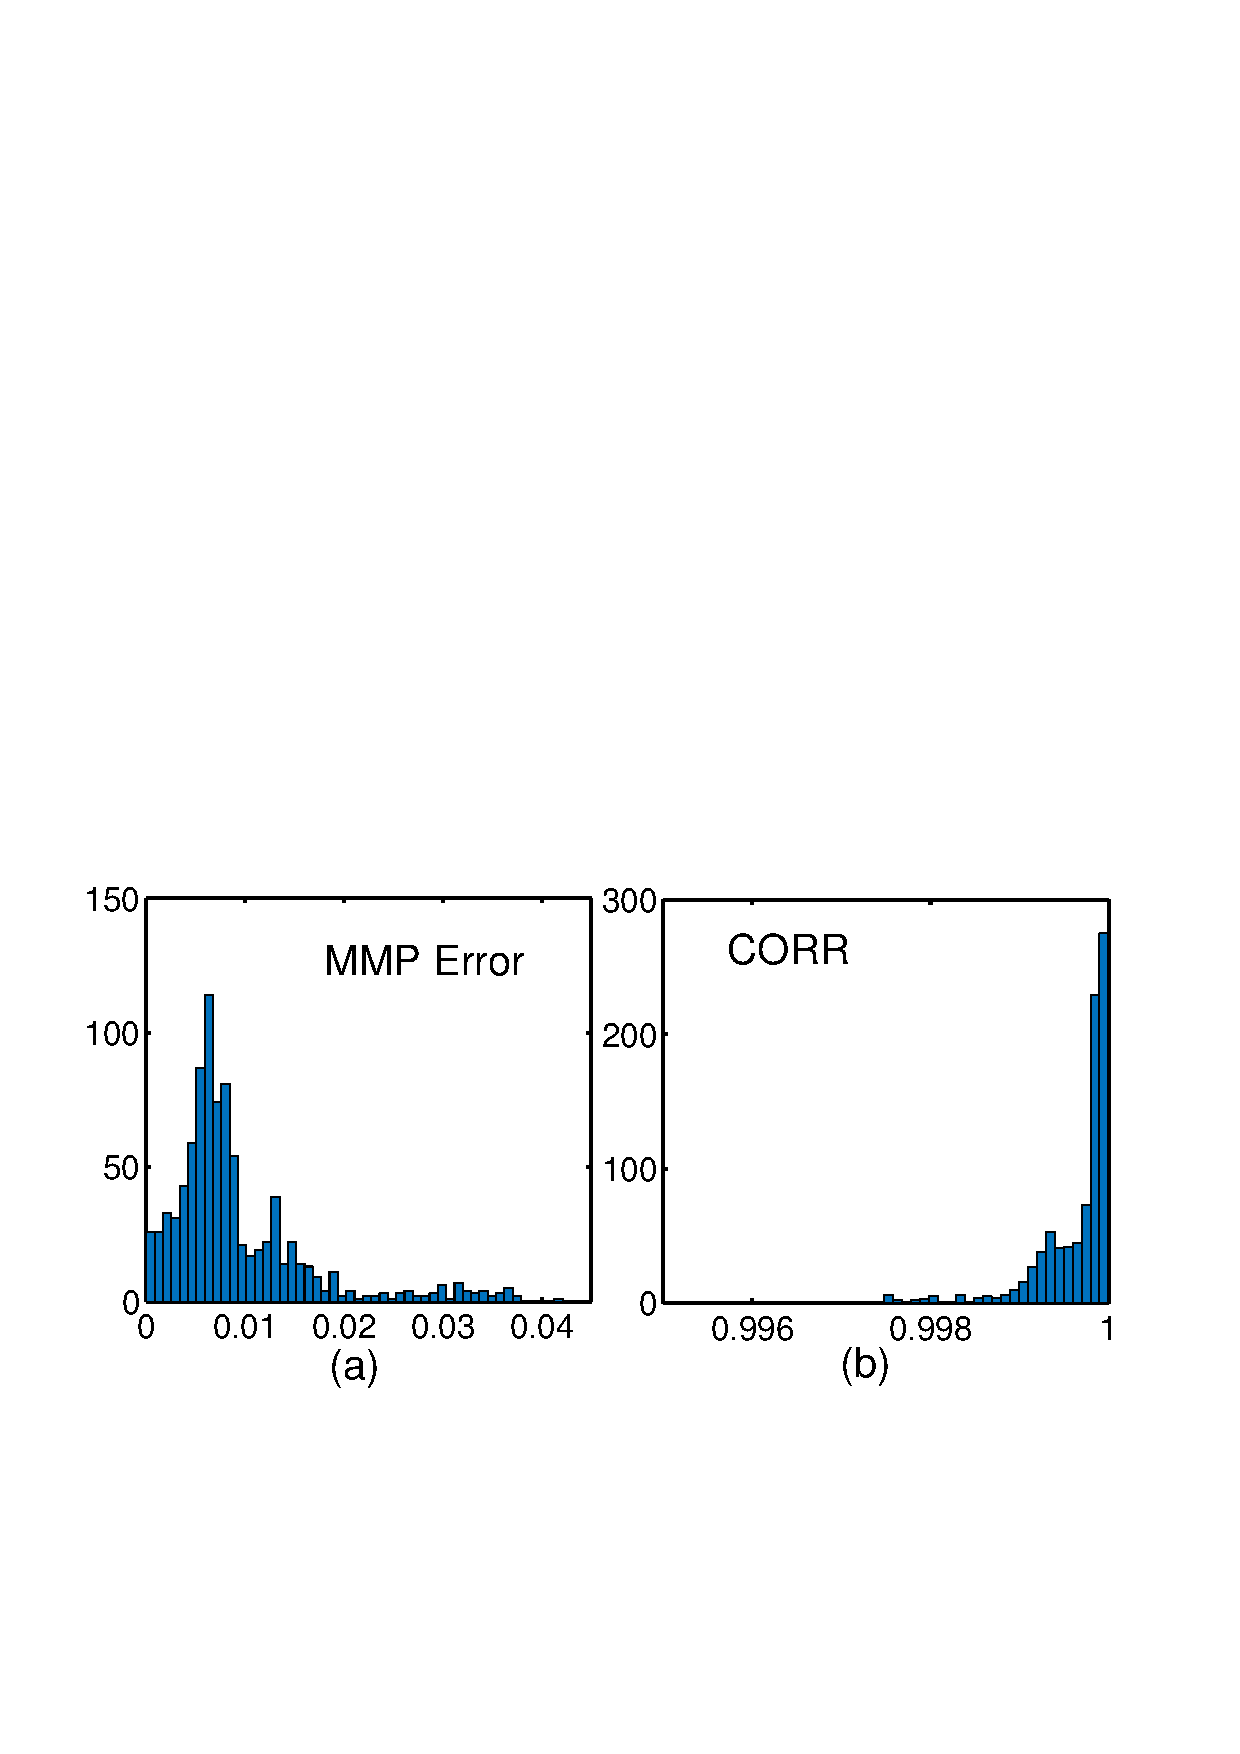
\includegraphics[width=1\columnwidth]{figs/cwHist_5lvl.pdf}
    \caption{(a) CW model's MPP error histogram over $900$ test cases (b) CW model's CORR histogram over $900$ test cases}
    \label{fig:cwHist}
\end{figure}

Figure \ref{fig:pvExample} shows an typical example of the P-V curves generated by the three models. The PV module is $60s2p$ with $3$ bypass diodes for each solar cell chain. Compared to the Ground Truth model's P-V curve (red solid line), the Colony-Wise model (blue dashed line) has almost the same accuracy, while the N-Colony model (green dot-dashed line) sacrifices the model a little bit to trade off for the constant computational speed.

First, we compare the Colony-Wise model with the Ground Truth model over the $900$ test cases. Figure \ref{fig:cwHist} (a) and (b) show the histogram of $900$ cases�� MPP error and CORR. The average MPP error is $0.92\%$, and the average CORR is $0.999$. In addition, the largest MPP error is $4.21\%$, $95\%$ of MPP errors are less than $2.60\%$, and the lowest CORR
is $0.995$. The results show that the Colony-Wise model has nearly the same accuracy as the Ground Truth model.

\begin{figure}[tb]
    \centering
    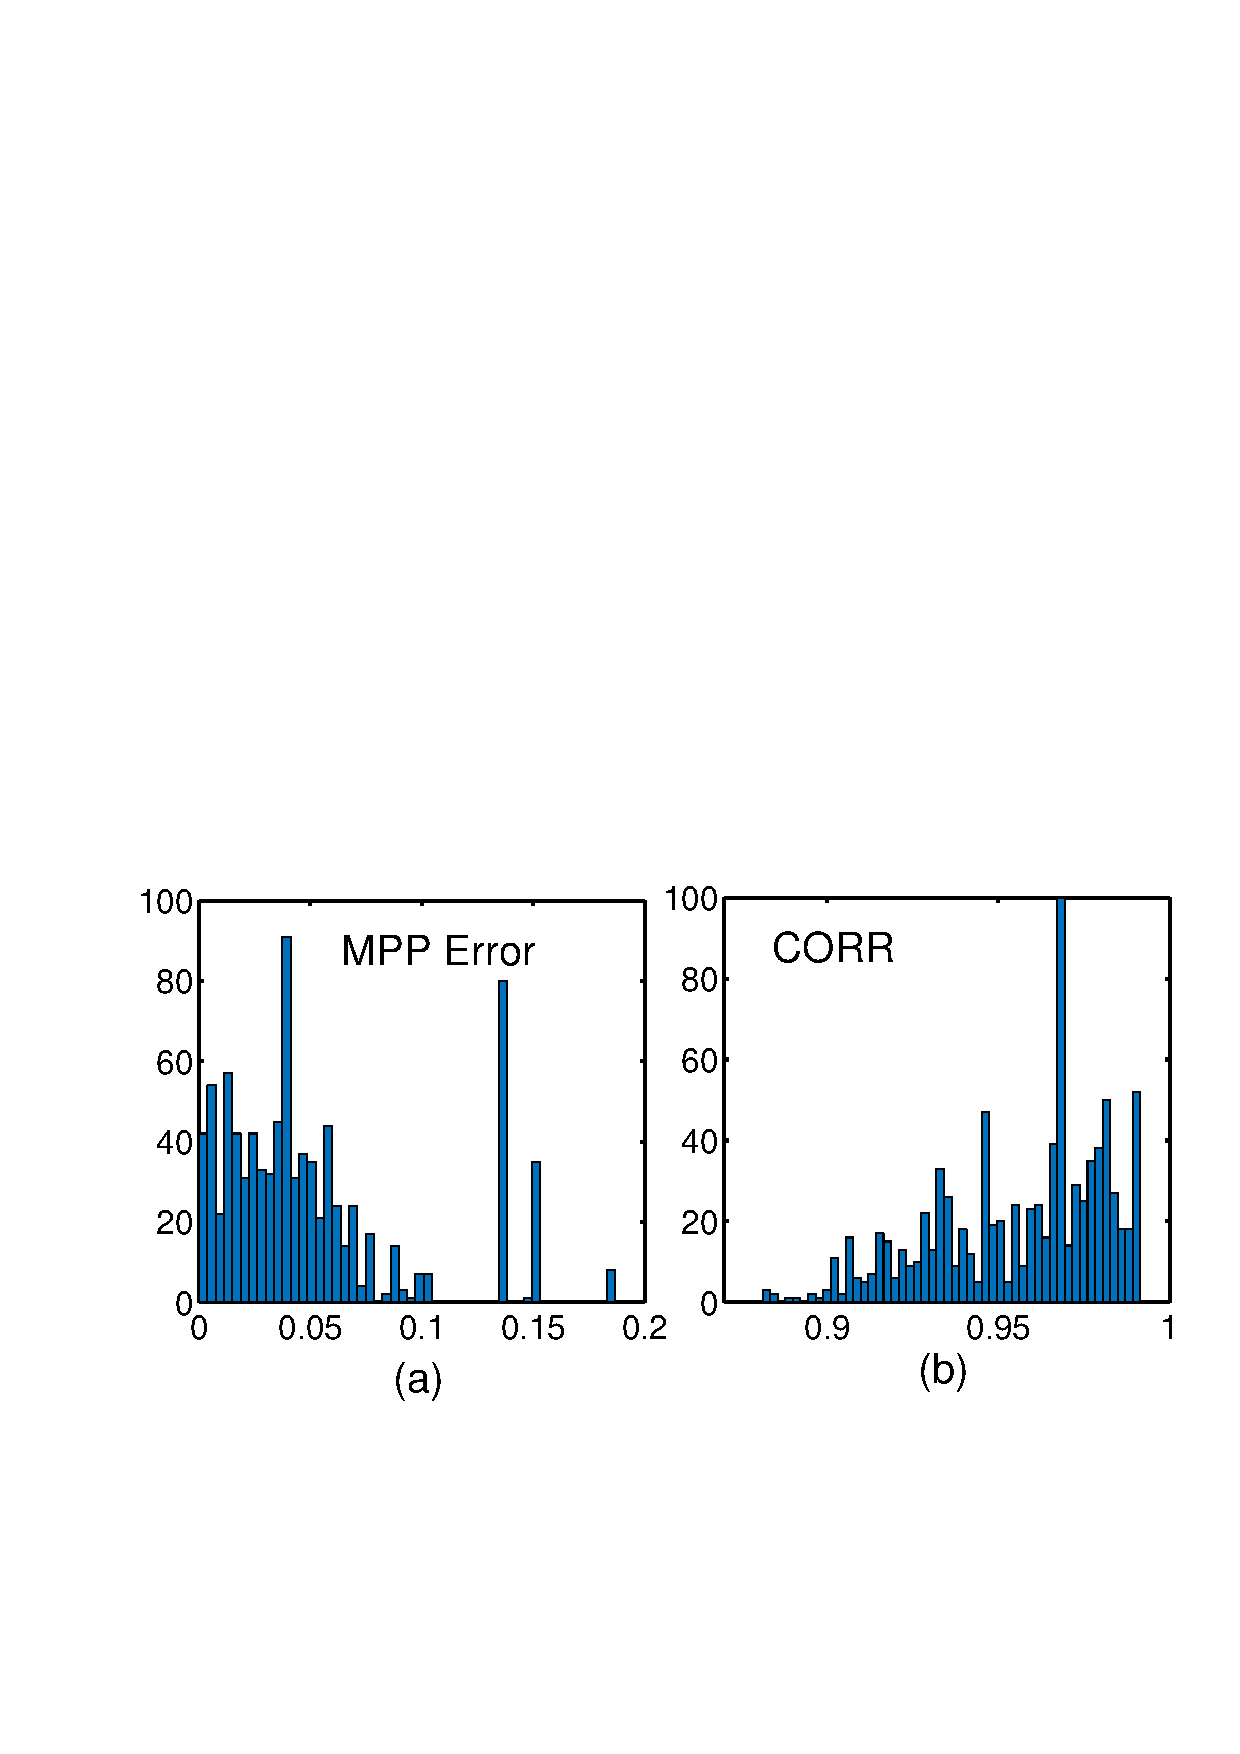
\includegraphics[width=1\columnwidth]{figs/ncHist_5lvl.pdf}
    \caption{(a) NC model's MPP error histogram over $900$ test cases (b) NC model's CORR histogram over $900$ test cases}
    \label{fig:ncHist}
\end{figure}

Then, we compare the N-Colony model with the Ground Truth model. Figure \ref{fig:ncHist} (a) shows the histogram of $900$ cases' MPP error, and (b) shows the CORRs' histogram. The average MPP error is $5.15\%$, and the average CORR is $0.96$. The NC model sacrifices the accuracy a little for it's constant computational complexity. There are two major reasons for the loss of accuracy. First, the NC model has constant number of circuit components. Therefore, there will be information loss when converting from the higher-ordered GT model to the lower-ordered NC model. Since the conversion is universal for one PV module type, the lost information is larger under some cases. Second, the NC model is an experimental model, which means some of its parameters are curved fitted (trained) through experiment data. Right now, we use $20$ patterns for training, and the model might suffer from over-fitting \cite{overfitting}. Therefore, the NC model has larger error for the cases that are not covered in the training set. To overcome this weakness, we can increase the number of training patterns.

\begin{table}[tb]
  \caption{Runtime of the Three Models}
  \label{table:rtComp}
  \centering
  \normalsize
\begin{tabular}{|l|l|l|l|}
  \hline
  \pbox{2cm}{PV Module \\ Config} & GT & CW (Speedup) & NC (Speedup)\\
  \hline
  $60s2p$ &$2216s$ & $318s$ (7.0X) & $129s$ (17.2X)\\
  \hline
  $30s4p$ &$1325s$ & $317s$ (4.2X) & $91s$ (14.5X) \\
  \hline
  $40s2p$&$1652s$ & $267s$ (6.2X) & $101s$ (16.3X) \\
  \hline
\end{tabular}
\end{table}


\subsection{Speed Comparisons Among the Three Models}
We compare the three models' efficiency in terms of HSPICE simulation time. The total run-time of the $300$ cases for each PV module is shown in Table \ref{table:rtComp}.

As shown in Table \ref{table:rtComp}, the average speedup of the Colony-Wise model and the N-Colony model are $5.8$X and $16$X. For each experiment configuration, the speedup roughly follows the diode ratio in Equation \ref{equ:diodeRatioGTCW} and \ref{equ:diodeRatioGTNC}.

The maximum speedup of the NC model is $17.2$X when the PV module setting is $60s2p$ ($3$ bypass diodes for each chain). The speedup can be higher when a PV module has more paralleled solar cell chain and more solar cells within each colony.
















